\documentclass[border=10pt]{standalone}

\usepackage{tikz}
\usepackage{tikzsymbols}
\usetikzlibrary{calc,patterns,shapes.geometric}

\def\centerarc[#1](#2)(#3:#4:#5){\draw[#1] ($(#2)+({#5*cos(#3)},{#5*sin(#3)})$) arc (#3:#4:#5);}

\begin{document}
	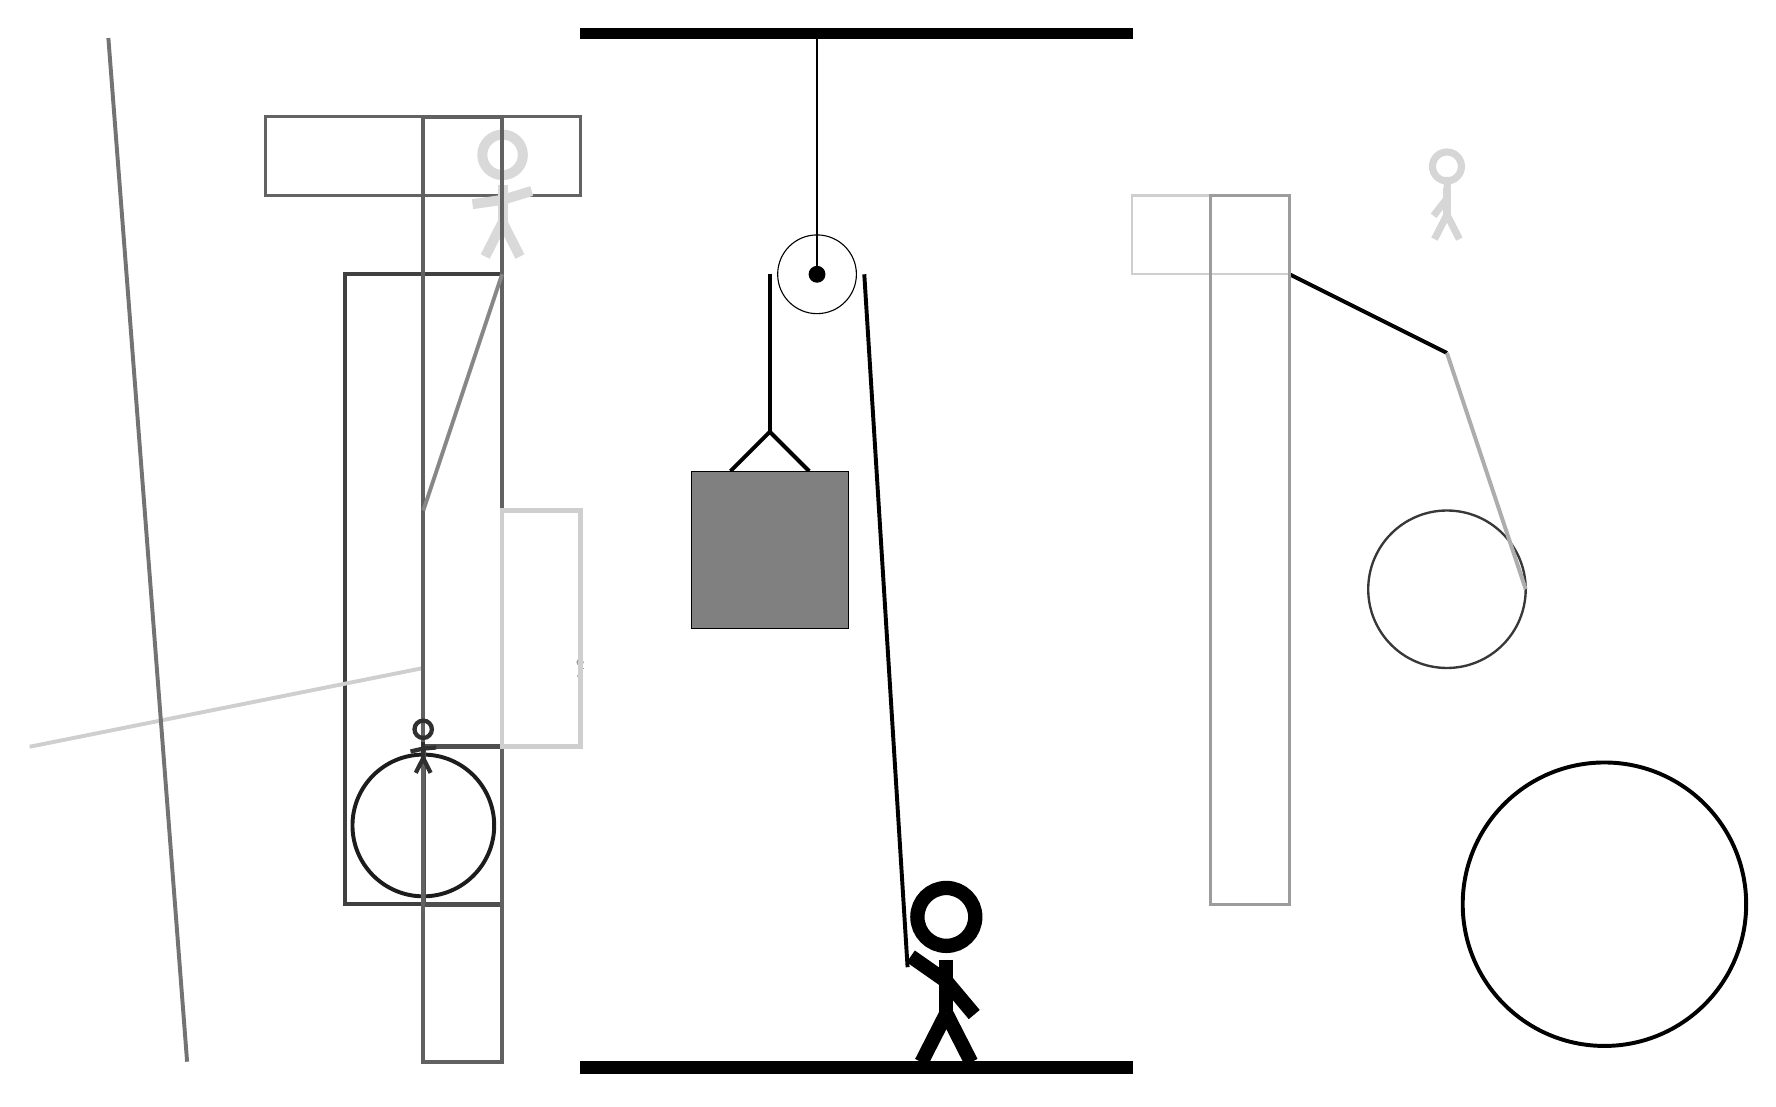
\begin{tikzpicture}
		%%%%% START %%%%%
		
		\draw[fill=black] (-2, 10) rectangle (5, 10.125);
		
		\draw (1, 7) circle (0.5);
		\draw[fill=black] (1, 7) circle (0.1);
		\draw (1, 10) -- (1, 7);
		
		\draw[line width=0.5mm] (-0.1, 4.5) -- (0.4, 5.0) -- (0.9, 4.5);
		\draw[fill=black!50] (-0.6, 4.5) rectangle (1.4, 2.5);
		
		\draw[line width=0.5mm] (0.4, 7) -- (0.4, 5.0);
		\centerarc[line width=0.5mm](1, 7)(0:180:0.6);
		\draw[line width=0.5mm](1.6, 7) -- (2.15, -1.8);
		
		\draw[line width=0.5mm, color=black!75] (-3, -1) rectangle (-5, 7);
		
		\draw[line width=0.5mm, color=black!98](7, 7) -- (9, 6);
		\draw [line width=0.5mm, color=black!89](-4, 0) circle (0.9);
		\draw[line width=0.6mm, color=black!69] (-4, -1) rectangle (-3, 1);
		
		\draw[line width=0.3mm, color=black!19] (7, 7) rectangle (5, 8);
		
		\draw[line width=0.5mm, color=black!19](-4, 2) -- (-9, 1);
		\draw[line width=0.4mm, color=black!61] (-2, 8) rectangle (-6, 9);
		
		\node[line width=0.4mm, color=black!15] at (-3, 8) {\Strichmaxerl[7][8][17]};
		\draw [line width=0.3mm, color=black!78](9, 3) circle (1.0);
		\draw[line width=0.5mm, color=black!62] (-4, -3) rectangle (-3, 9);
		
		\draw[line width=0.5mm, color=black!47](-3, 7) -- (-4, 4);
		\node[line width=0.7mm, color=black!39] at (-2, 2) {\Strichmaxerl[1][84][0]};
		\draw[line width=0.6mm, color=black!19] (-2, 4) rectangle (-3, 1);
		\draw [line width=0.5mm, color=black!100](11, -1) circle (1.8);
		\node[line width=0.5mm, color=black!81] at (-4, 1) {\Strichmaxerl[3][13][5]};
		\draw[line width=0.5mm, color=black!55](-7, -3) -- (-8, 10);
		\draw[line width=0.5mm, color=black!32](9, 6) -- (10, 3);
		\draw[line width=0.4mm, color=black!39] (6, 8) rectangle (7, -1);
		\node[line width=0.5mm, color=black!16] at (9, 8) {\Strichmaxerl[5][52][89]};
		
		
		\node at (2.6, -1.9) {\Strichmaxerl[10][-35][-50]};
		
		\draw[fill=black] (-2, -3) rectangle (5, -3.15);
		
		%%%%% END %%%%%
	\end{tikzpicture}
\end{document}